\section{Introducción}
	\subsection{Motivación}
	En el vertiginoso avance de la tecnología, la aplicación de redes neuronales en el procesamiento de imágenes ha emergido como un catalizador revolucionario en diversas disciplinas. Entre las múltiples facetas que abarca esta amalgama de inteligencia artificial y visión computarizada, la detección y clasificación de señales de tránsito se destaca como un campo de estudio de gran relevancia e impacto práctico.
La seguridad vial es una preocupación global de suma importancia, y el tráfico vehicular se presenta como un escenario dinámico y complejo donde la correcta interpretación de señales juega un papel crucial. La detección automatizada y la clasificación precisa de señales de tránsito no solo pueden potenciar la eficiencia de los sistemas de transporte, sino que también desempeñan un papel esencial en la prevención de accidentes y la mejora de la movilidad urbana.
	\begin{figure}[ht]
		\centering
		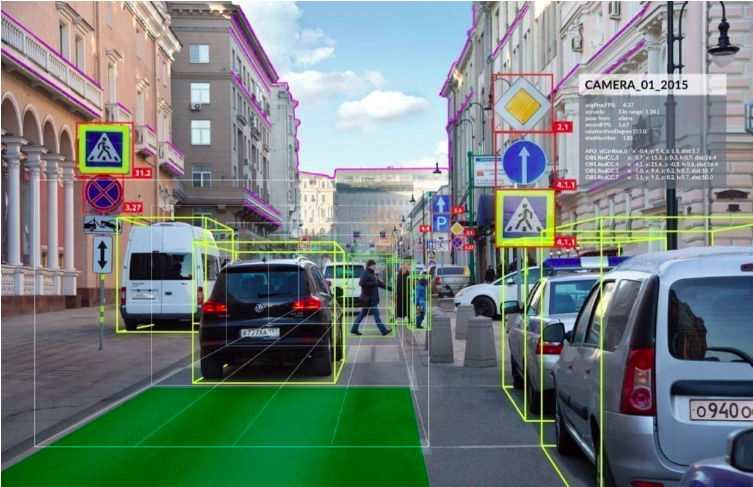
\includegraphics[height=7cm]{3}
		\caption{Reconocimiento de Objetos.}
	\end{figure}
	
El crecimiento exponencial de datos visuales en entornos urbanos y la necesidad de respuestas rápidas ante señales cambiantes hacen imperativa la adopción de enfoques avanzados. Acá es donde las redes neuronales toman importancia, porque su capacidad para aprender patrones complejos a partir de grandes conjuntos de datos permite el desarrollo de modelos capaces de discernir con precisión las señales de tráfico en imágenes, incluso en condiciones adversas.
En este contexto, la motivación subyacente es impulsar la aplicación de redes neuronales en el ámbito específico de la detección y clasificación de señales de tránsito.

\subsection {Objetivo}
\newpage

\section{Marco Teórico}
\section{Implementación}
\section{Resultados}
\section{Conclusión}
\section{Bibliografía}
